\chapter{The Eclipse IDE}\label{cha:TheEclipseIDE}

In the following chapter a general overview of Eclipse framework and its most prominent components is provided. A description and analysis of available plugins from which essential information could be captured is presented. Last but not least a great amount of focus is given on a specific plugin which is used and enhanced throughout the thesis.  

\todo{ide eclipse plugins, available what are useful, present all, write adv and dis. describe contextual factors that can be achieved, describe how programmers work within this ide. }
\todo{focus on rabbit specia chapter explain why to choose that, positive negative, limitations. provide class diagram and explanation, name the issues}

\section{Eclipse}
\label{sec:TheEclipseIDE:eclipse}
Eclipse framework is an IDE fairly used by several developers: to primarily develop Java applications, to also develop in other programming languages via plugins, and to develop documents and packages for other softwares. 
The standard SDK Eclipse distribution contains a base workspace with certain functionalities, Java Developemnt tooling plug-ins and layout. Thereafter additional plug-ins allow the extension of the workspace, and Eclipse can become a multifunction framework to be used for: Embedded programming, C++ programming, javaBeans, Java application, websites, or even develop additional Eclipse plugins, etc. The plug-ins can be removed or replace according to the needs of the developer.

Eclipse framework is an open platform for integrating tools, editors, views and plug-ins. Its source code is freely available and anyone can contribute by builting their own new plug-ins or by engaging in discussions regarding integrated tools. 

\section{Menus, views and editors}

When starting up Eclipse, either a welcoming screen greets the developer if its a newly initiated or the previously workspace is loaded otherwise. Figure \ref{fig:eclipse_worspace} displays a standard Eclipse setup, a java integrated development environment. Eclipse's main window is called the \textit{workbench} and based on the active \textit{perspective} its appearance is defined. A perspective has its own a set of elements views and editors and menus along with a adaptable personalised layout for specific tasks such as debugging a program. 
\label{sec:TheEclipseIDE:menusviewsandeditors}
	\begin{figure}[!ht]
		\begin{center}
			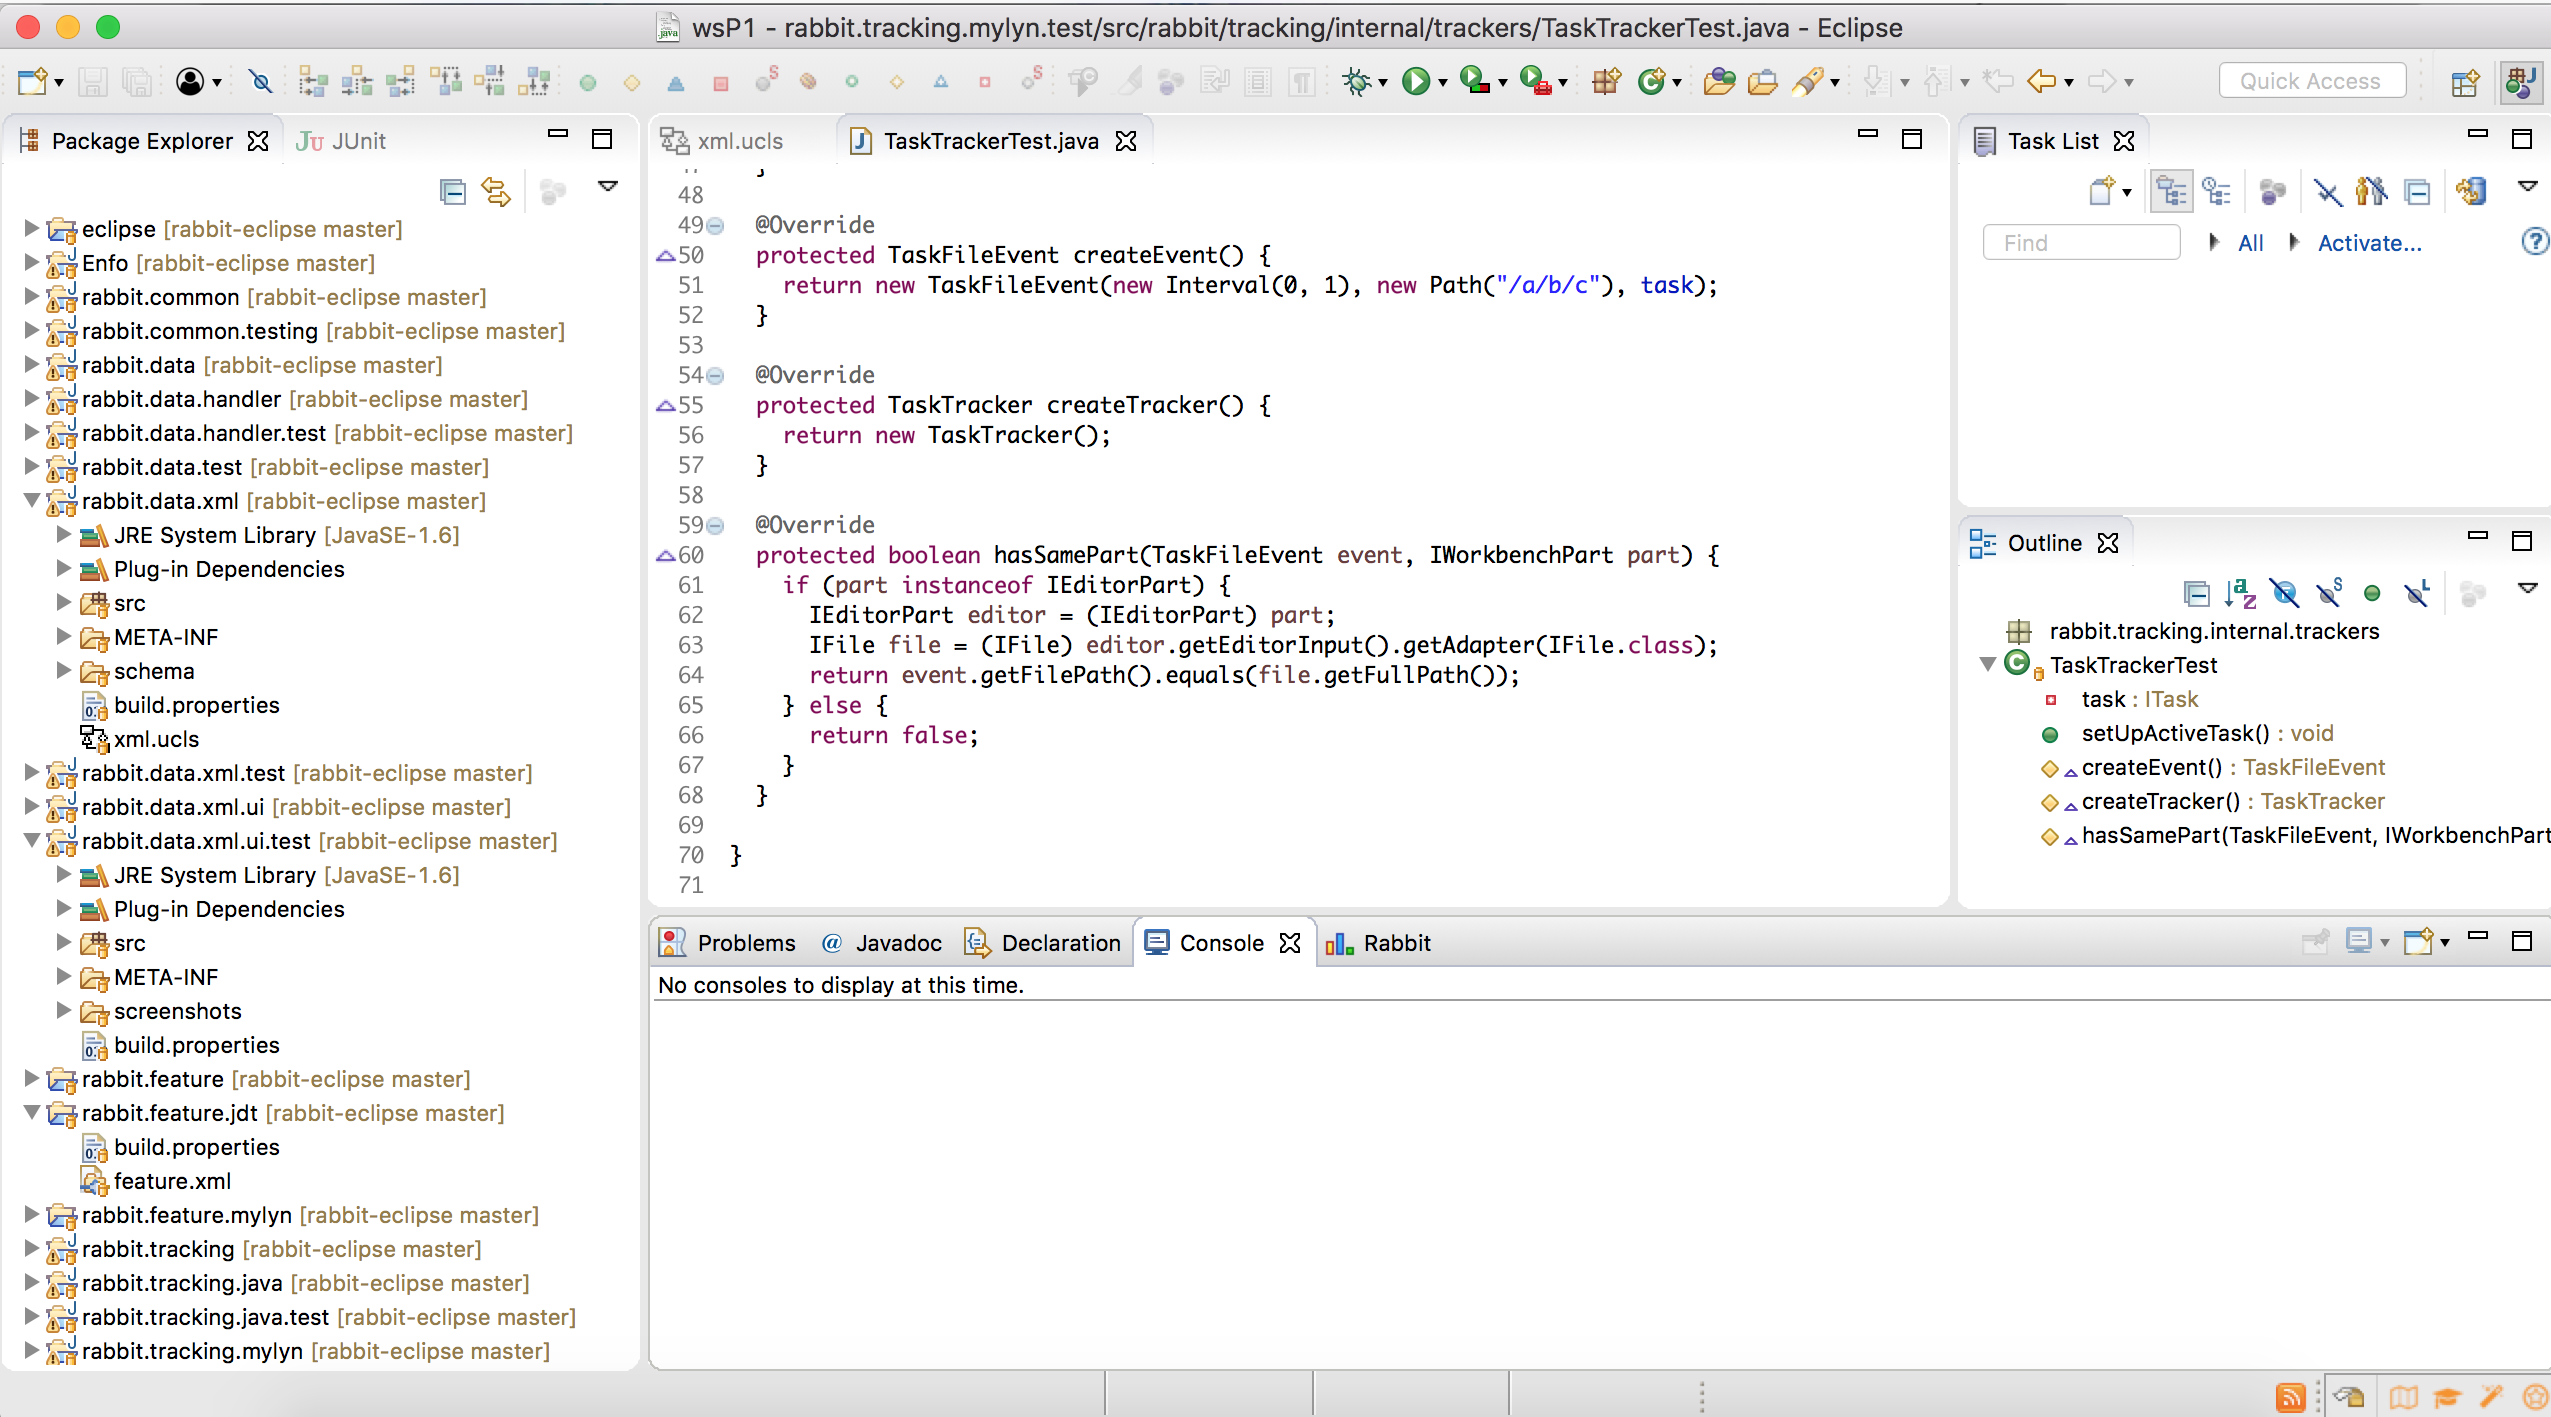
\includegraphics[width=\textwidth]{figures/eclipse_workspace.png}
		\end{center}
		\caption{The Java Development perspective in Eclipse.}
		\label{fig:eclipse_workspace}
	\end{figure}
A view is a window that enables the developer to examine something, eclipse offers various of views f.x. Java packages and their files. An editor is a smart editor which recognises the programming language markups the syntax and allows you to modify and save files. Editors share characteristics with views, but unlike views, editors don't have toolbars. Eclipse is filled up with menus and toolbars, the main menu is at the top of the screen while views and explorers usually provide their own context menus.




\section{Plug-ins}
\label{sec:TheEclipseIDE:plugins}
Eclipse is a multifunction framework and it provides several software components (plug-ins). By using the Plug-in Developer Environment (PDE) developers can either extend Eclipse IDE by creating new additional functionalities for plug-ins or even improve and extend the capabilities of already implemented plug-ins. When a plugin is installed the platform dynamically discovers the registered plug-ins and invokes them when they are needed.

Although the reason Eclipse provides this thumping range of tools to support the developer, usually instead a chaotic environment is generated. For this reason several researchers and developers instrumented plug-ins to understand developers' workflow. These plug-ins are mostly observing the usage of Eclipse artifacts and record the activity and the interactions of a developer. The most commonly used plug-ins are listed. 

\section{the focus for rabbit}
\label{sec:TheEclipseIDE:rabbit}
